\chapter{適用例}\label{cha:Indication}
本章では、本研究で提案した手法が正しく動作することを確認する。
適用例として、本提案手法を適用する帳票画像を、以下の図\ref{fig:indication_original}に示す。
図\ref{fig:indication_original}に対して、本提案手法を適用し、出力であるJSON形式のファイルとPNG形式の画像を確認する。

\begin{figure}[t]
    \begin{center}
        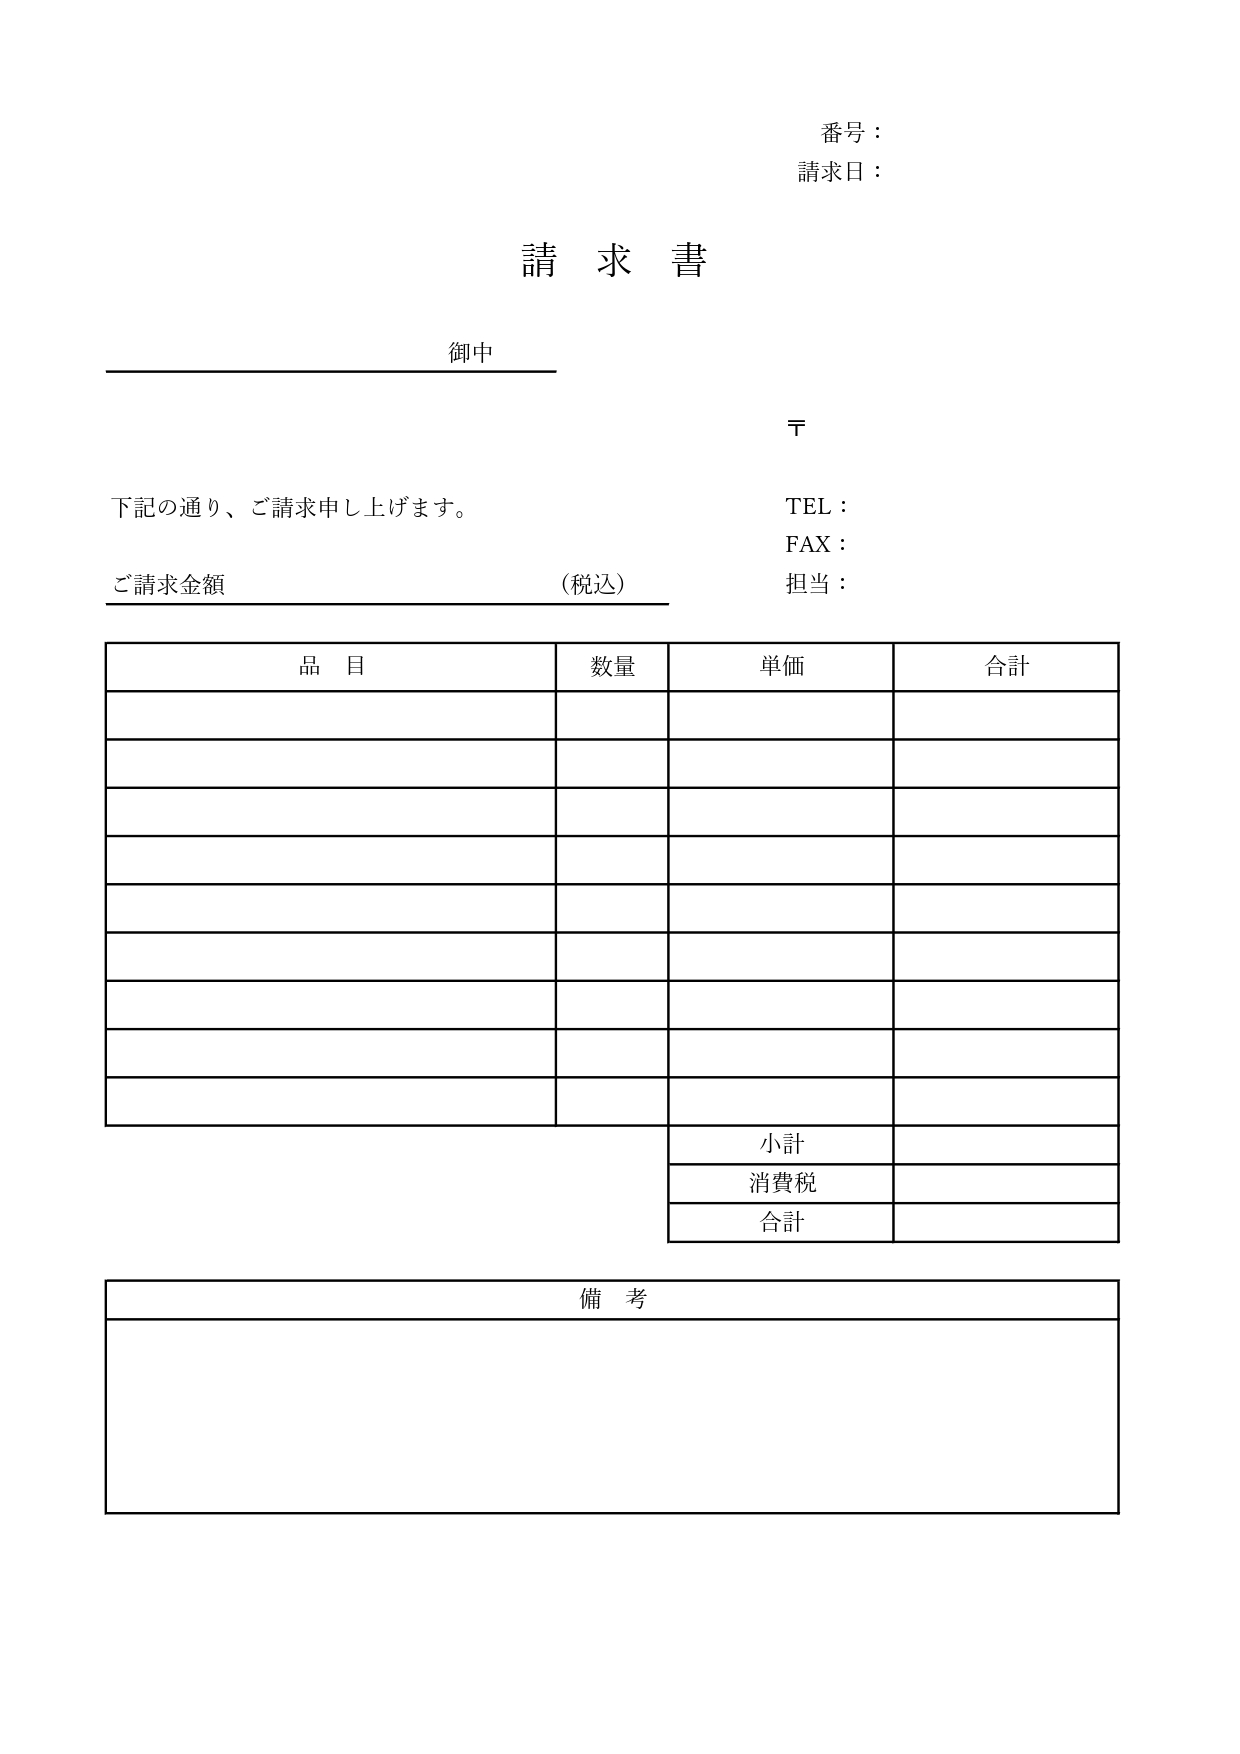
\includegraphics[width=15cm]{image/05-indication/indication_original.jpg}
        \caption{本提案手法を適用する帳票画像}
        \label{fig:indication_original}
    \end{center}
\end{figure}


\section{JSON形式のファイルの出力結果}\label{sec:result_json}
図\ref{fig:indication_original}の帳票画像に対して、本提案手法を適用し、出力したJSON形式のファイルの一部を以下の図\ref{fig:exported_json}に示す。

\begin{figure}[t]
    \begin{center}
        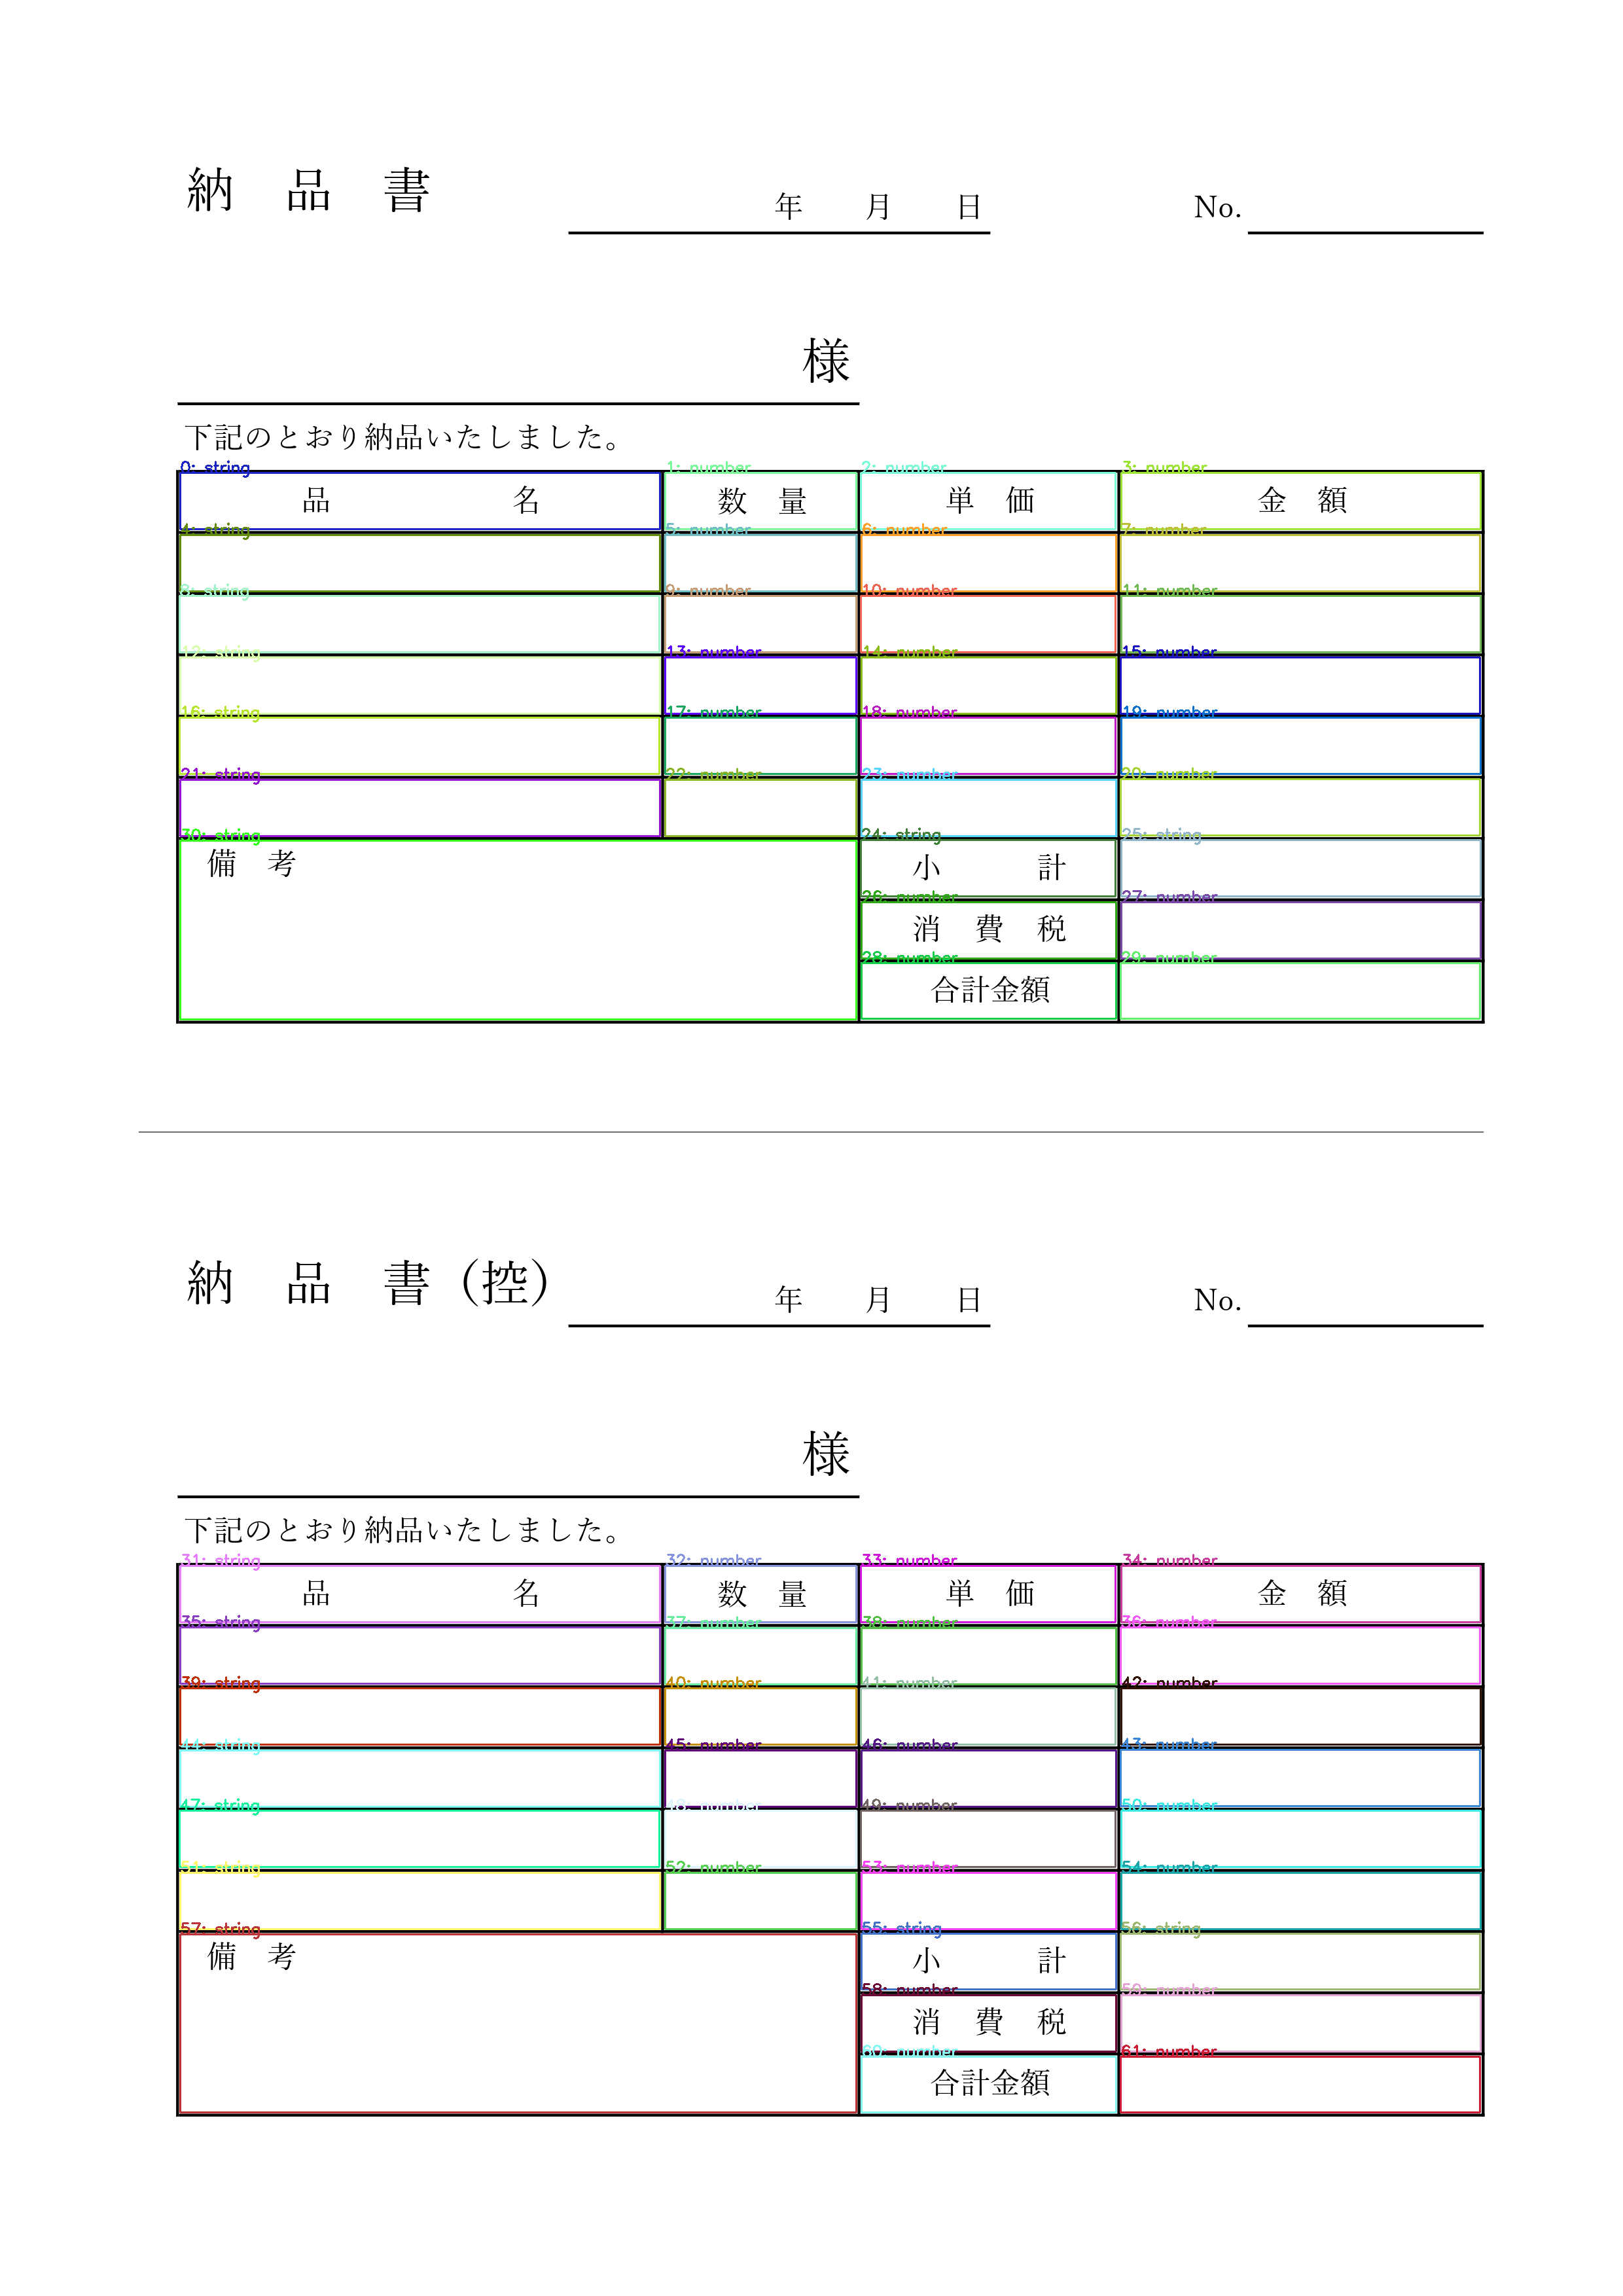
\includegraphics[width=15cm]{image/05-indication/rects_with_label.png}
        \caption{図\ref{fig:indication_original}に本提案手法を適用し、出力したJSON形式のファイルの一部}
        \label{fig:exported_json}
    \end{center}
\end{figure}


\section{領域強調画像出力機能の出力結果}\label{sec:result_OCR}
図\ref{fig:indication_original}の帳票画像に対して、本提案手法を適用し、出力したPNG形式の画像を以下に示す。

\begin{figure}[t]
    \begin{center}
        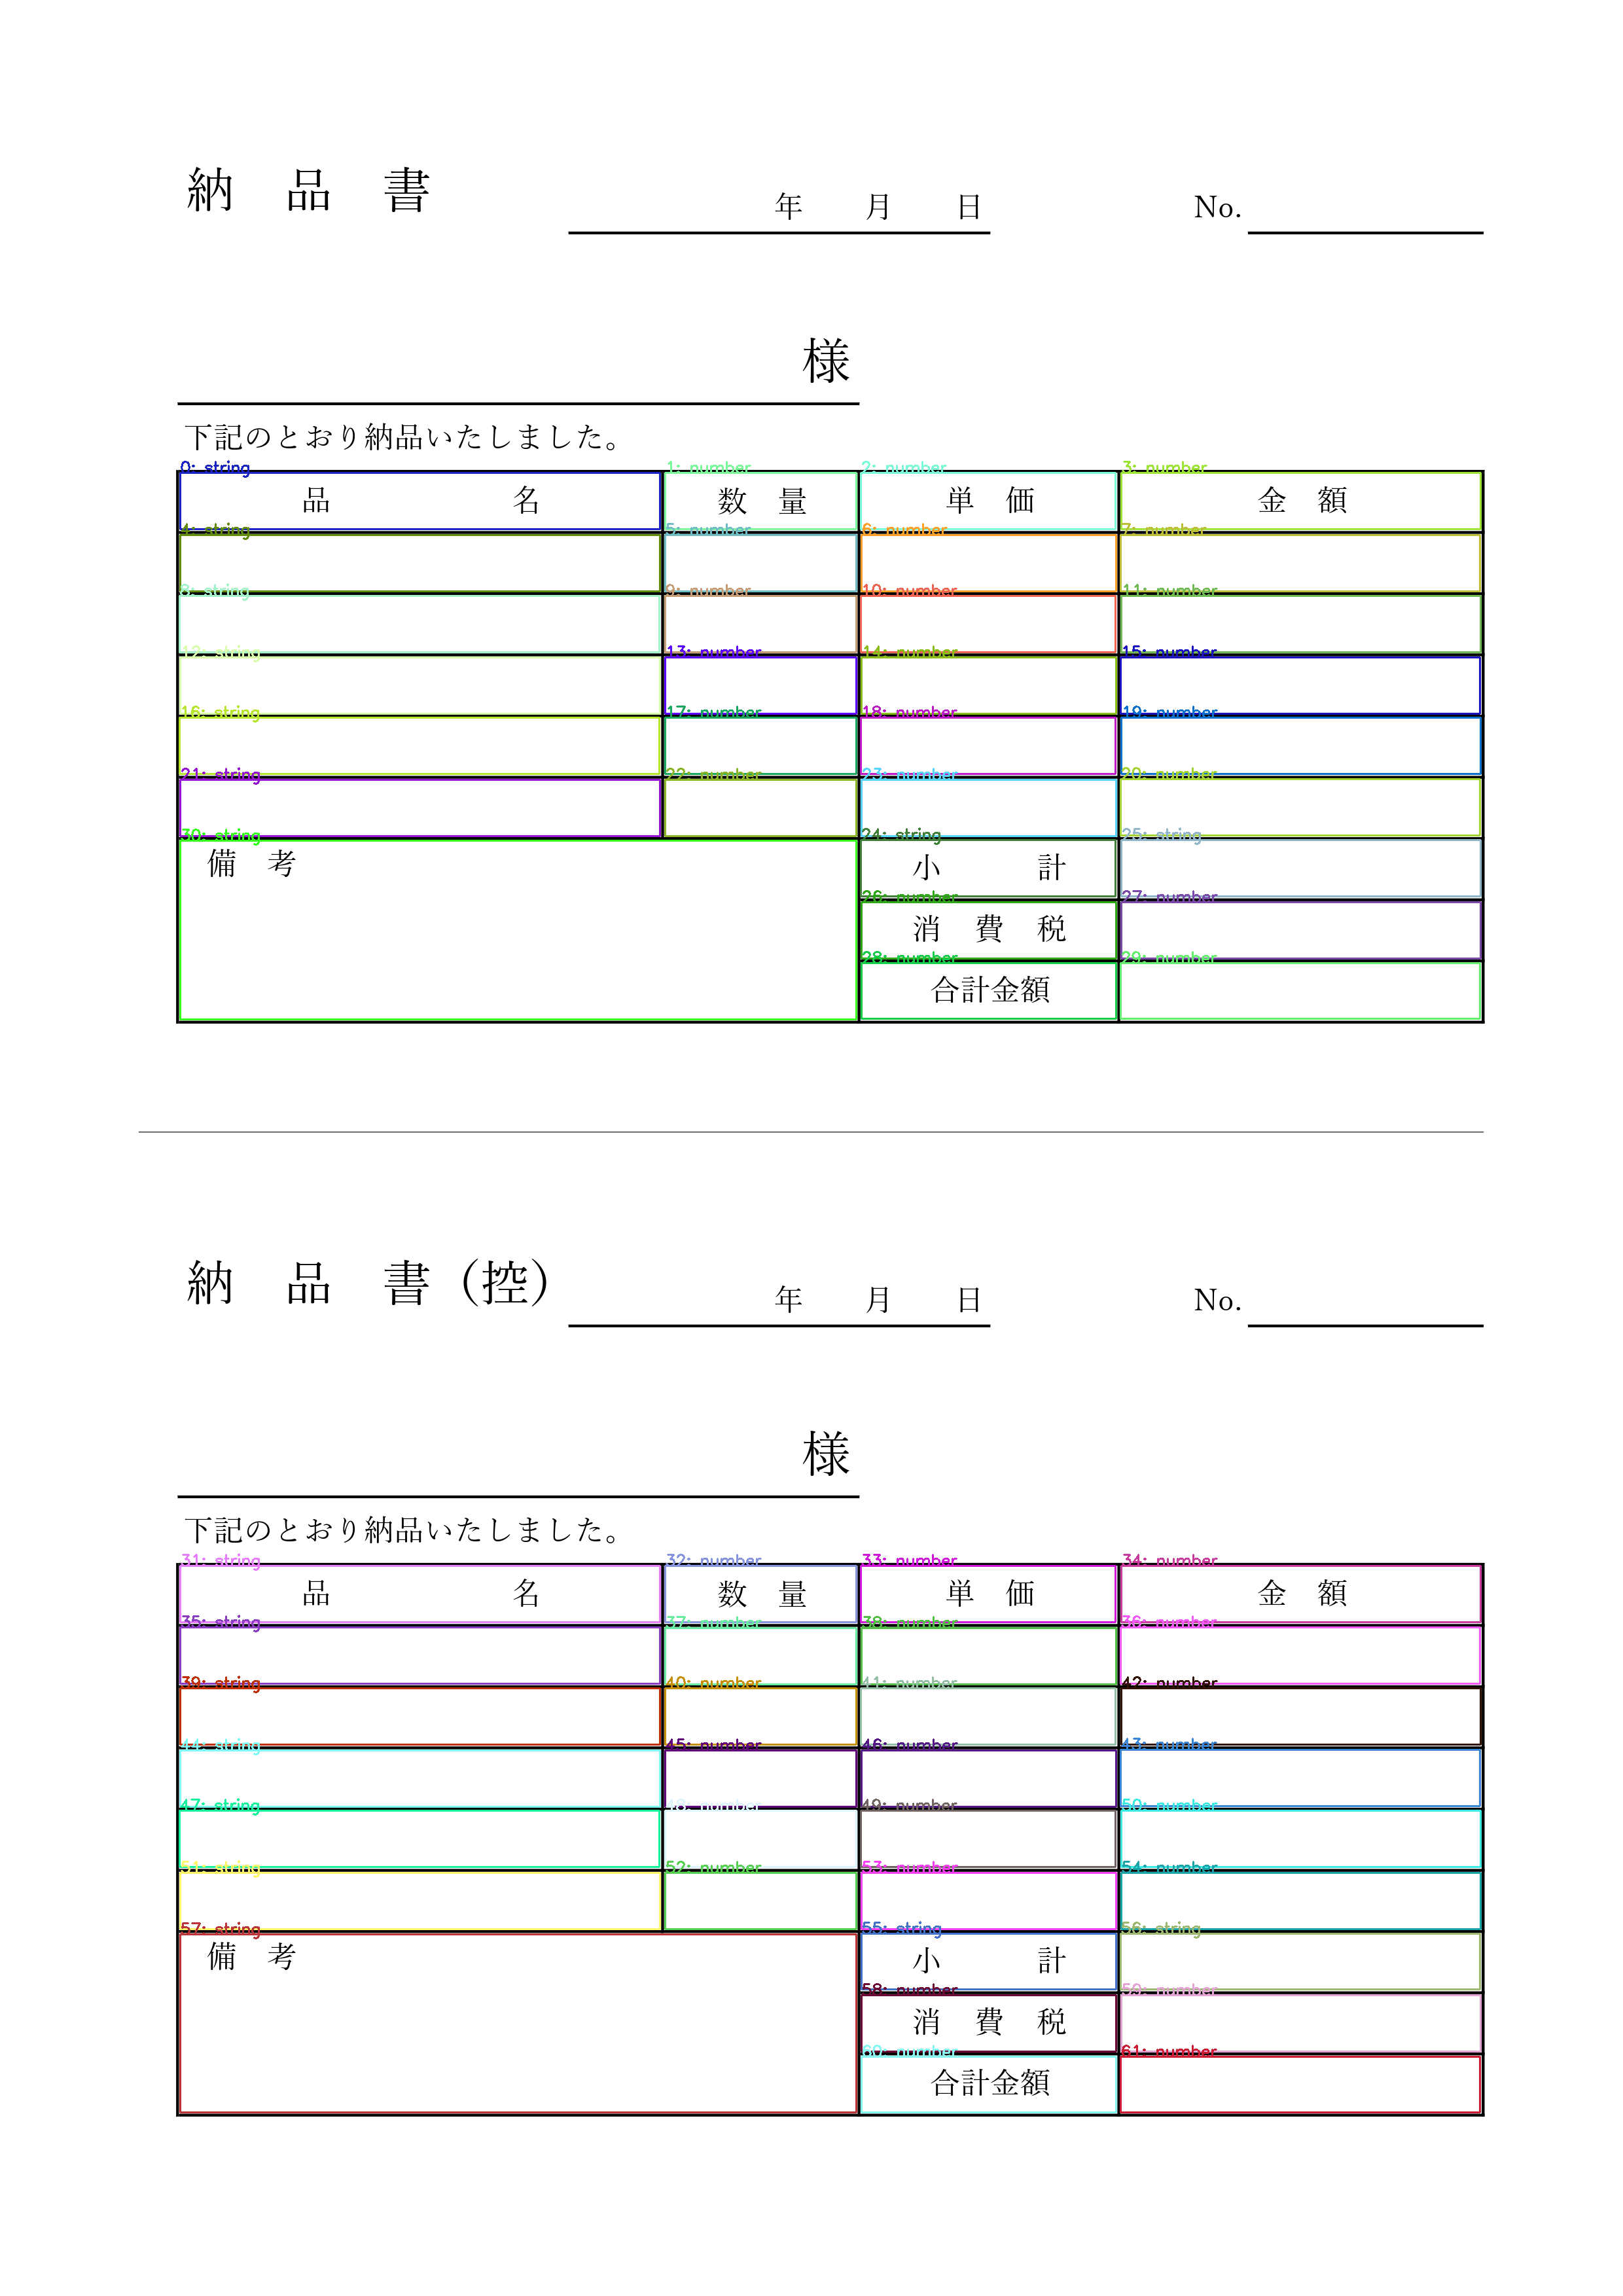
\includegraphics[width=15cm]{image/05-indication/rects_with_label.png}
        \caption{図\ref{fig:indication_original}に本提案手法を適用し、出力した矩形領域強調画像}
        \label{fig:exported_png}
    \end{center}
\end{figure}